%===============================================================================
% ifacconf.tex 2022-02-11 jpuente  
% Template for IFAC meeting papers
% Copyright (c) 2022 International Federation of Automatic Control
%===============================================================================
\documentclass{ifacconf}

\usepackage{graphicx}
\usepackage{natbib} 

\begin{document}
\begin{frontmatter}

\title{Android Content Providers in Mobile Distributed Computing \thanksref{footnoteinfo}} 

\thanks[footnoteinfo]{Velbazhd Software LLC}

\author[First]{Gergana Mateeva} 
\author[First]{Dimitar Parvanov} 
\author[Second]{Ioan Dimitrov} 
\author[First]{Iliyan Iliev}
\author[First]{Todor Balabanov} 

\address[First]{Bulgarian Academy of Sciences\\Institute of Information and Communication Technologies\\acad. Georgi Bonchev Str., block 2, 1113 Sofia, Bulgaria\\(gergana.mateeva, dimitar.parvanov, iliyan.iliev, todor.balabanov) @iict.bas.bg}
\address[Second]{Technical University of Sofia\\Faculty of Electronic Engineering and Technology\\8 St. Kliment Ohridski Blvd., block 1, 1756 Sofia, Bulgaria\\joancdimitrov@tu-sofia.bg}

\begin{abstract}
Distributed computing and volunteer computing became very popular in the last two decades. Both are used for problems easily separable for simultaneous calculations on many heterogeneous machines. The only difference is that volunteer computing has been done on a donated calculating power. With the rise of smart mobile devices, volunteer computing appeared in the world of mobile distributed computing. With its capabilities, Android OS became an attractive environment for such computations. Android's Content Providers became a valuable tool for information transfer in mobile distributed computing applications. 
\end{abstract}

\begin{keyword}
Android, distributed computing, volunteer computing
\end{keyword}

\end{frontmatter}

\section{Introduction}

Fast after its appearance mobile distributed computing become a part as state of the art in the soft computing \cite{Angelova-2009-a} and even more with Covid-19 pandemic \cite{Petrov-2021-a}. The ideas applied in the wireless sensor networks \cite{Alexandrov-2016-a} has been influenced the ideas of computations distribution on mobile devices and even integration with IoT \cite{Dineva-2019-a} with smart routing \cite{Tashev-2019-a}. Splitting calculations in heterogeneous devices appears to be efficient in complex problems like combinatorial problems \cite{Borissova-2015-a}. Having calculations on devices under somebody else control \cite{Balabanov-2020-a} except advantages also rises many cybersecurity issues \cite{Dimitrov-2021-a}.

Distributed computing is appropriate for a limited number of computational problems. The main characteristic which the problem should have is the possibility of different calculation steps being calculated separately. Also, it is important that different calculation results have less need for synchronization between the calculating nodes. Parallel implementation of the QuickSort algorithm \cite{Sanders-1997-a}, for example, is not suitable for distributed computing. Splitting of the array between the calculating nodes needs synchronization. The final result of the algorithm needs synchronization too. Problems like parallel QuickSort are more suitable for multiprocessor systems with tight control over calculations and communication. Parallel evolutionary algorithms \cite{Sudholt-2015-a}, on the other side, are appropriate for a very high degree of parallelization and a very low need for synchronization. This fact makes them a perfect candidate for distributed computing even on less powerful mobile devices. 

Most of the evolutionary algorithms are fast computed themselves \cite{Vural-2012-a}. The difficulties come when the target function (fitness function) is computationally time-consuming \cite{Di-Pietro-2004-a}. Most evolutionary algorithms need many calculations of the target function in order to try different candidate solutions. When the target function is very time-consuming so many calculations make the optimization process practically unusable \cite{Lee-2015-a}. 

The paper is organized as follows: Section 1 introduces mobile distributed computing and its specifics; Section 2 presents a practical implementation and the usage of embedded functionality; Section 3 concludes and provides some guidance for further research. 

\section{Android Content Providers}

\begin{figure}
\begin{center}
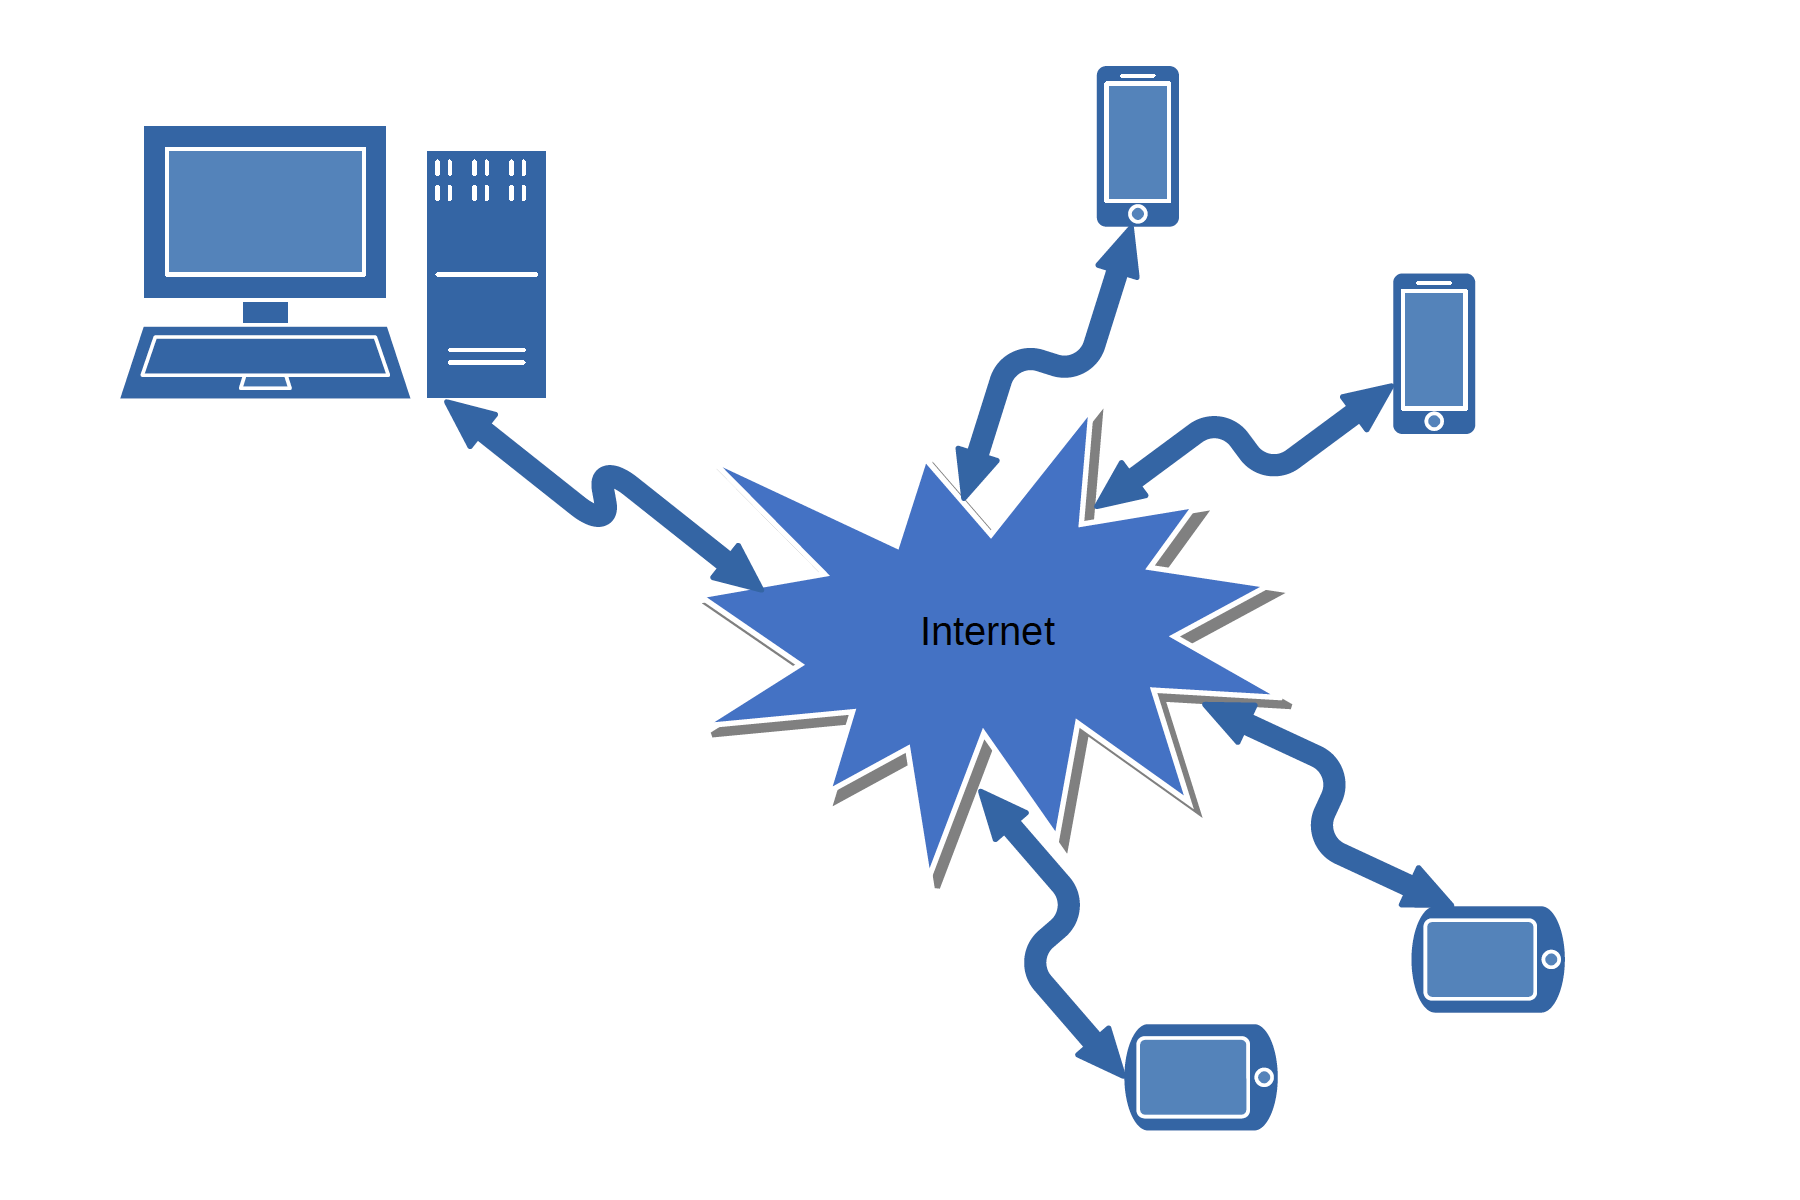
\includegraphics[width=8.4cm]{images/fig0001}
\caption{Client-server architecture} 
\label{fig0001}
\end{center}
\end{figure}

Vitosha Trade Android Client \cite{Balabanov-2016-1} is a distributed computing client application for Android. The project was created during HackTogether competition, held October 1-2, Sofia/Bulgaria, 2016 and it is developing in the Institute of Information and Communication Technologies as part of the Bulgarian Academy of Sciences. The project is doing time-series forecasting by training artificial neural networks with gradient-based methods \cite{Tomov-2021-a} and evolutionary algorithms \cite{Tomov-2021-b}. The forecasting is done on Android mobile devices as background calculations organized with the Android Service component and the active wallpaper capabilities of the operating system \cite{Mateeva-2021-a}. 

\begin{figure}
\begin{center}
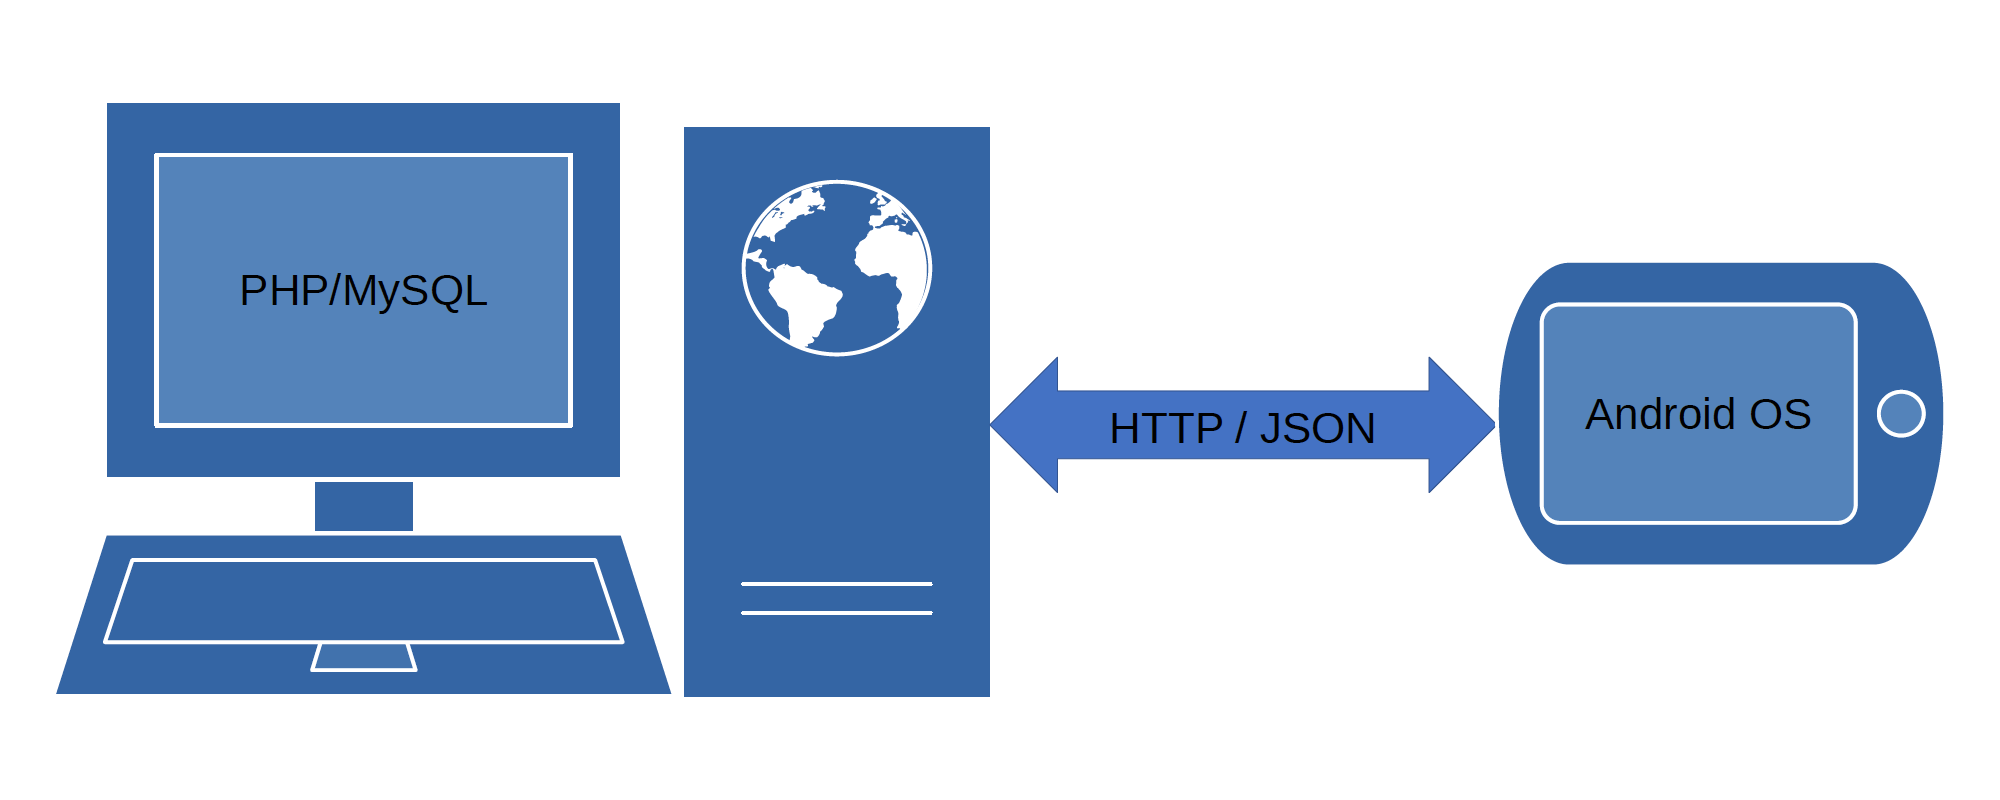
\includegraphics[width=8.4cm]{images/fig0002}
\caption{HTTP communication} 
\label{fig0002}
\end{center}
\end{figure}

The system is organized on the client-server principle. Time series are presented on a lightweight web server (Fig. \ref{fig0001}). Each mobile device connects to the server through the Internet and obtains calculation packages. The communication is done over HTTP/JSON protocol (Fig. \ref{fig0002}). Training of the artificial neural networks is done in a separate forecasting module (Fig. \ref{fig0003}). Such separation is very useful for multi-interface implementation. Not only is the rich graphical interface of Android OS, but the system also supports a simplified command-line interface. In this way, machine learning algorithms can be evaluated outside of the complicated Android environment simply running desktop command-line implementation. 

\begin{figure}
\begin{center}
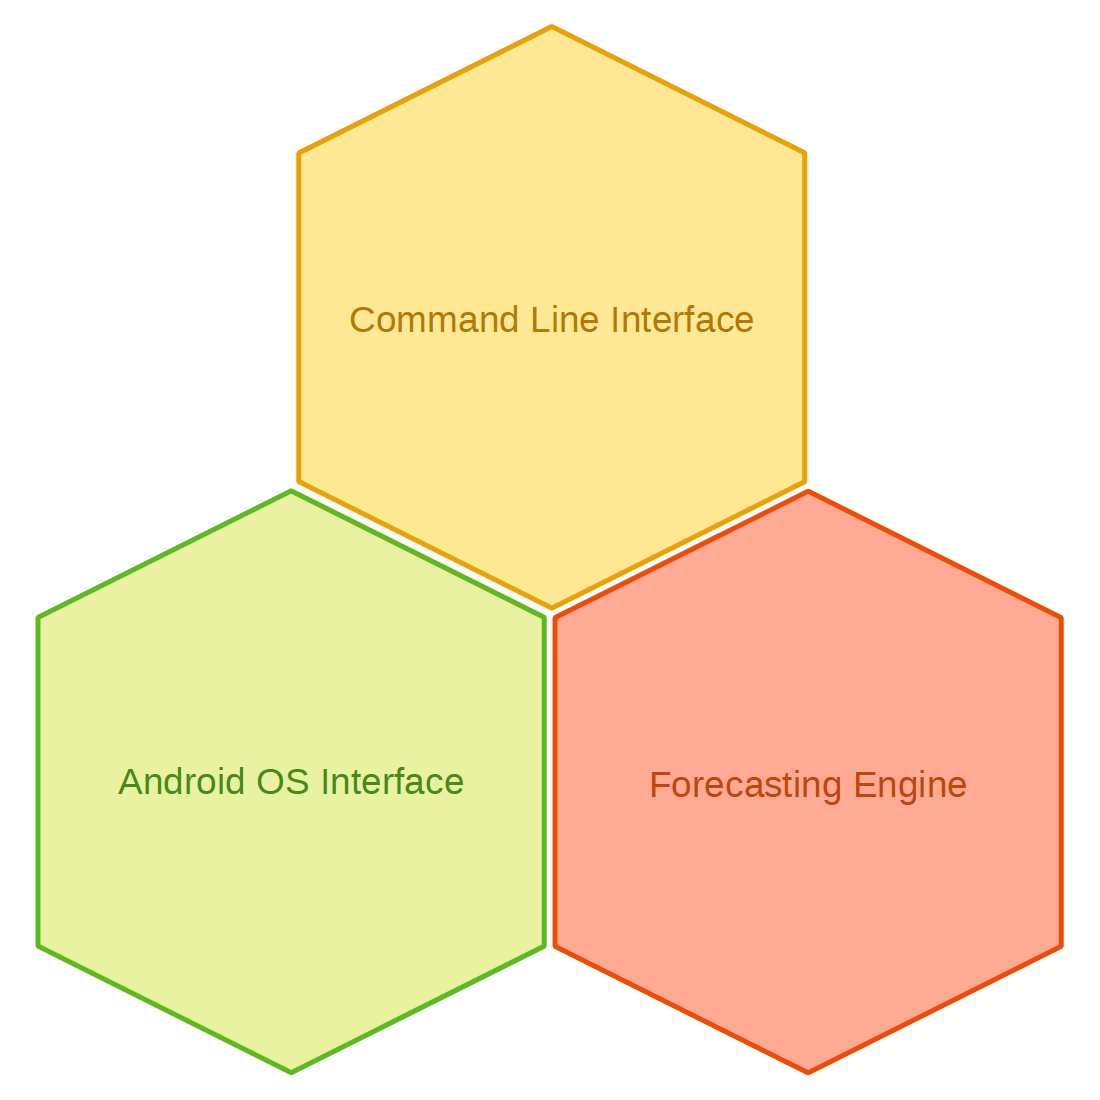
\includegraphics[width=8.4cm]{images/fig0003}
\caption{Modular architecture} 
\label{fig0003}
\end{center}
\end{figure}

Inside the Android module of the system, there is another separation according to data flow needs. The forecasting engine module is called in the background by the Android Service component. This action is done on idle usage of the mobile device. During artificial neural networks training, time series are disassembled on training examples (Fig. \ref{fig0004}). Cycles of gradient-based and evolutionary optimization over the network's weights are performed (Fig. \ref{fig0005}). At the end of each training session, a forecast is generated. At this point, Android Content Providers come in place. Such a Content Provider is used for storing the generated forecast inside the local SQLite database. The visualization part of the system is organized as Live Wallpaper and Widgets.

\begin{figure}
\begin{center}
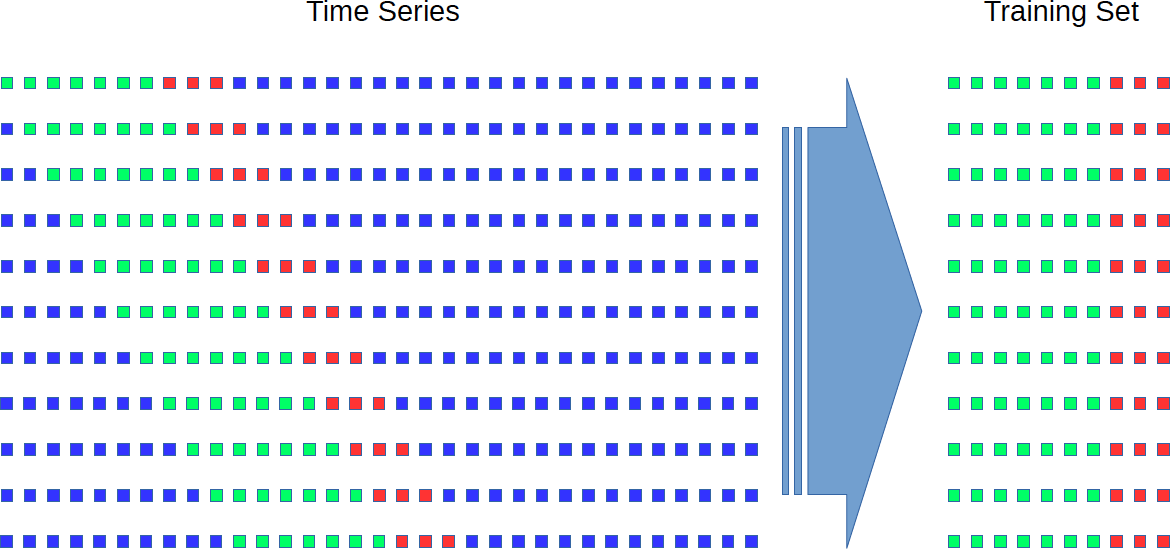
\includegraphics[width=8.4cm]{images/fig0004}
\caption{Training set formation} 
\label{fig0004}
\end{center}
\end{figure}

\begin{figure}
\begin{center}
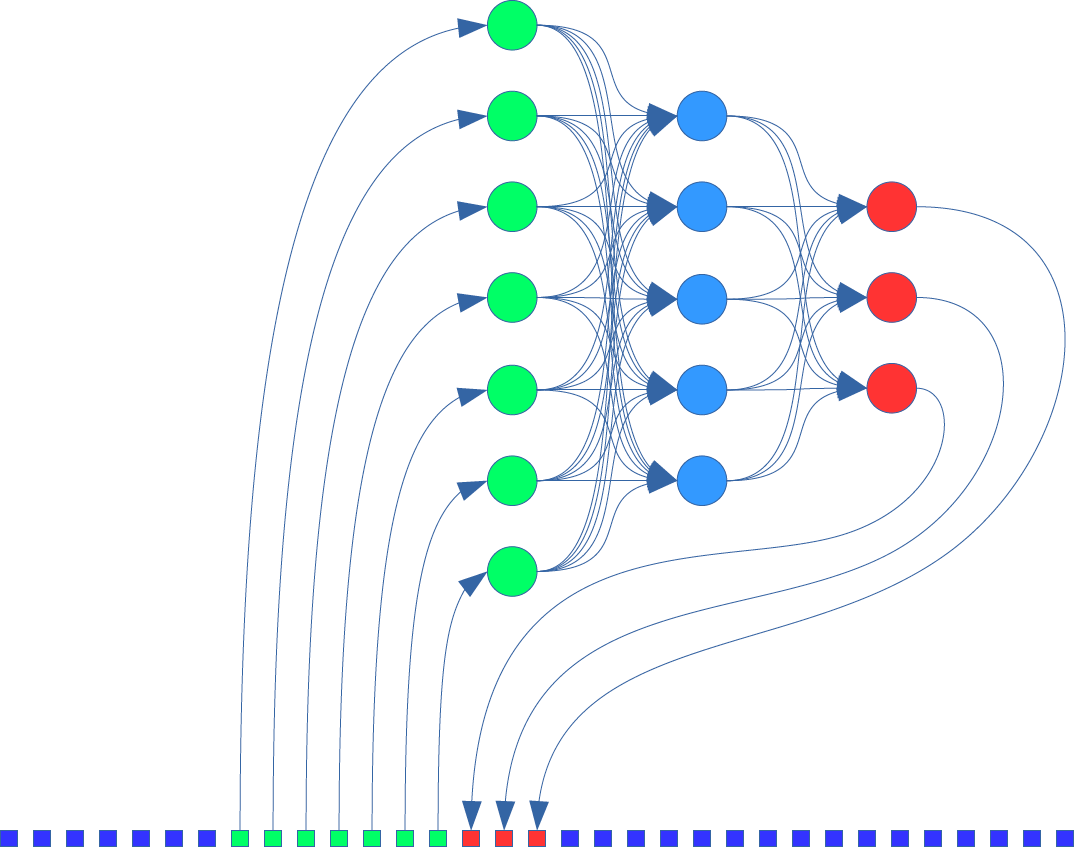
\includegraphics[width=8.4cm]{images/fig0005}
\caption{Artificial neural network data feeding} 
\label{fig0005}
\end{center}
\end{figure}

The Live Wallpaper shows three types of information. The first area is for the time series ticker and time interval.  The second area is a simplified topology of the artificial neural network. The third area is a simplified time series forecast. All these areas are available as visual widgets. Most of the visualization is pixel drawing. For better efficiency and for unified data access Android Content Providers are used once again. Forecast generation is a time-consuming process and appears asynchronously. That is why it is very rational for the forecast to be stored by Content Provider immediately after its generation and to be obtained by Content Provider each time when visualization is needed. 

Voting capabilities of the system are the third place where Content Providers come in place. Voting is part of human-computer distributed computing \cite{Tomov-2019-a}. The user has a separate Android Widget for its voting. Pressing the arrow-up or arrow-down the vote is handled by the Content Provider. The Content Provider helps with the voting control because the user is allowed to vote only once in a particular time series interval. 

\section{Conclusion}

By using Android Content Providers mobile distributed computing becomes more efficient. Content Providers improve the application modularity and robustness. Having the Content Providers allows for better integration of the application with the operating system and with the other applications. 

As further research, other consumers of the proposed Content Providers can be developed and approved.

\begin{ack}
This research is funded by Velbazhd Software LLC. It is partially supported by the Ministry of Education and Science of the Republic Bulgaria under the National Science Program “Intelligentanimal husbandry”, grant agreement No. D01-62/18.03.2021/, the National Research Programme “Young scientists and postdoctoral students” approved by DCM No. 577/17.08.2018, and the Bulgarian National Science Fund by the project “Mathematical models, methods and algorithms for solving hard optimization problems to achieve high security in communications and better economic sustainability”, KP-06-N52/7/19-11-2021.
\end{ack}

\bibliography{references}

\end{document}
